\section{Hydrogen burning through four trillion years}\label{sec:hydrogen}

\subsection{The three long-term tracks}
Tracks S, F and P start from the same kind of static hydrogen-burning model
and differ in nuclear network and composition transport
(Table~\ref{tab:ingredients}). Figure~\ref{fig:hr} shows all three in the
HR diagram with the LBA97 track; Figure~\ref{fig:composition} shows the
composition and convection histories. Table~\ref{tab:milestones} lists the
computed milestones by track.

\begin{figure}[H]\centering
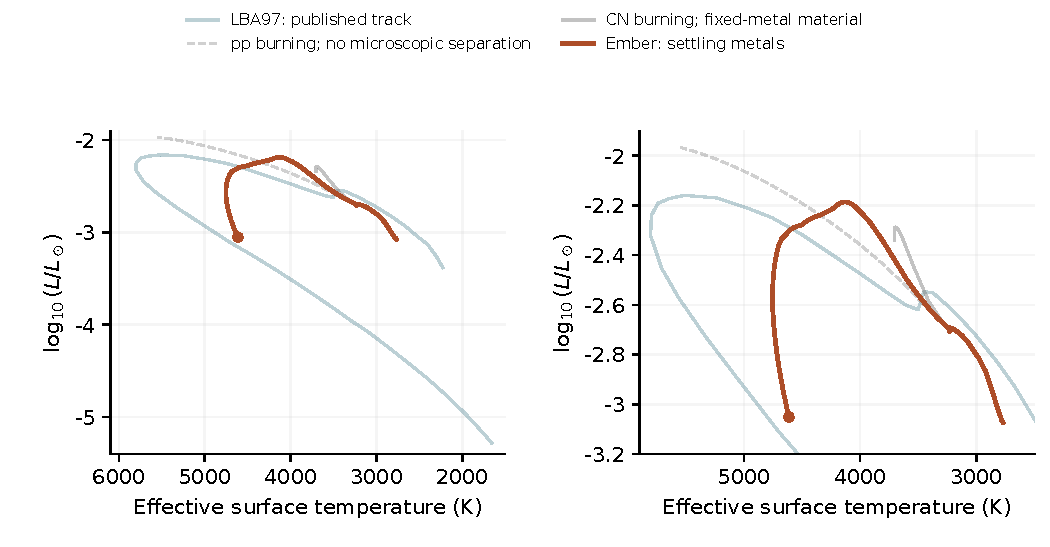
\includegraphics[width=\textwidth]{lba97_hr.pdf}
\caption{HR diagrams of Track S (orange, through $4.002\Tyr$), Track F
(solid gray, through $3.704\Tyr$), Track P (dashed gray, through
$3.890\Tyr$) and the published LBA97 track (pale blue, read from its
Figure~1 without age rescaling). Left: full range; right: the
hydrogen-burning portion. Track P differs from S in both nuclear and
transport physics, so the separation between them is not the effect of
settling alone. The small luminosity dip near 3230 K accompanies the
formation of an interior radiative layer.}
\label{fig:hr}
\end{figure}

\begin{table}[H]\centering\small
\caption{Computed milestones. Ages in Tyr on the long-term clock; ``---''
means not reached or not recorded for that track.}\label{tab:milestones}
\begin{tabular}{@{}lrrr@{}}\toprule
Event & Track S & Track F & Track P \\\midrule
Maximum central $^3$He (mass fraction) & --- & --- & 0.7103 (0.1003) \\
Loss of full convection (central $X$) & $\simeq3.55$ & 3.549 (0.1744) & 3.546 (0.1751) \\
Centre becomes radiative & 3.551 & 3.551 & --- \\
Central $X=10^{-3}$ & 3.650 & 3.661 & --- \\
Central $X=10^{-4}$, $10^{-5}$ & 3.660, 3.767 & --- & --- \\
Luminosity maximum ($\Ls$; $\Teff$) & 3.673 (0.006513; 4128 K) & 3.677 (0.005163; 3695 K) & --- \\
Surface-temperature maximum & 3.838 (4754 K) & 3.689 (3705 K) & --- \\
Last computed model & 4.002 & 3.704 & 3.890 \\
\quad $\Teff$ (K) & 4612 & 3702 & 5546 \\
\quad central $X$ & $3.528\times10^{-8}$ & $1.309\times10^{-4}$ & $8.157\times10^{-4}$ \\
\quad surface $X$ & 0.9982 & 0.8905 & 0.1730 \\
\quad convective mass fraction & 0.01553 & --- & 0.02565 \\
\quad nuclear share of luminosity & 97.28\% & --- & --- \\\bottomrule
\end{tabular}
\end{table}

At its endpoint Track S has $R=0.04667\Rs$, $L=0.0008881\Ls$, central
temperature 6.443 MK, central density $3.982\times10^4$ g cm$^{-3}$,
central metal fraction 0.1312, surface metal fraction below $10^{-40}$,
and $0.003797\Ms$ of hydrogen remaining. Surface temperature has declined
by 141.5 K over the 164.3 Gyr since its maximum, but hydrogen burning still
supplies 97.28\% of the light; the model has turned toward cooling but is
not yet on a passive cooling sequence.

\begin{figure}[H]\centering
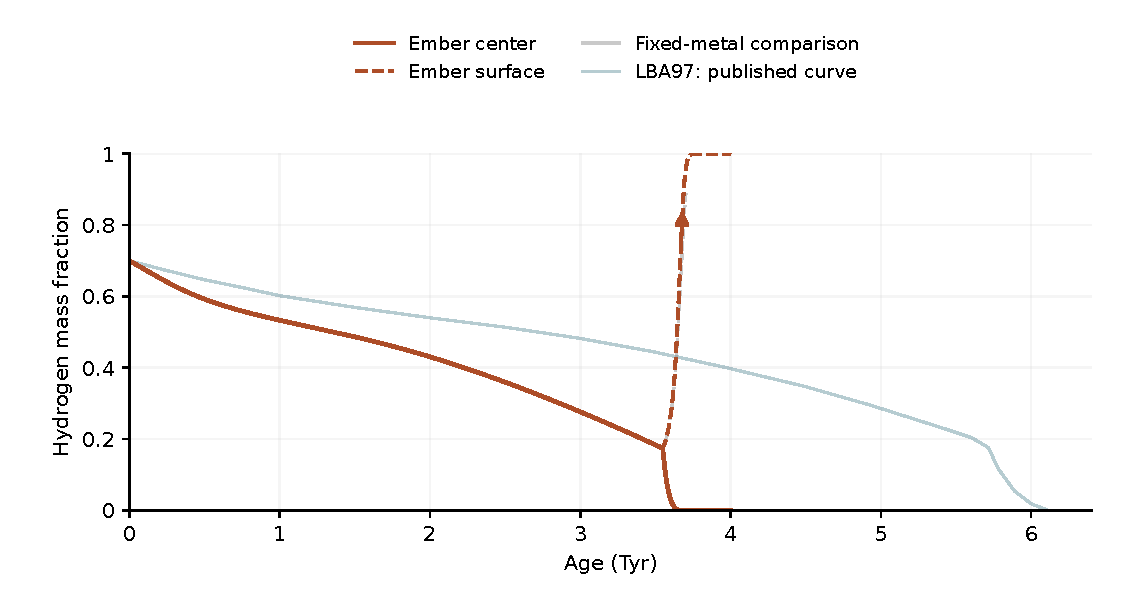
\includegraphics[width=0.7\textwidth]{hydrogen_evolution.pdf}\\[2pt]
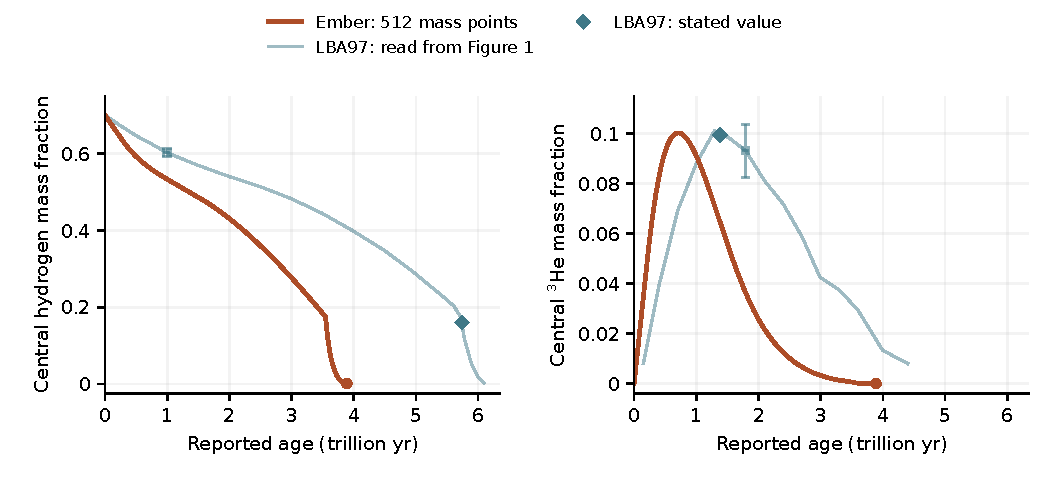
\includegraphics[width=0.7\textwidth]{lba97_composition.pdf}\\[2pt]
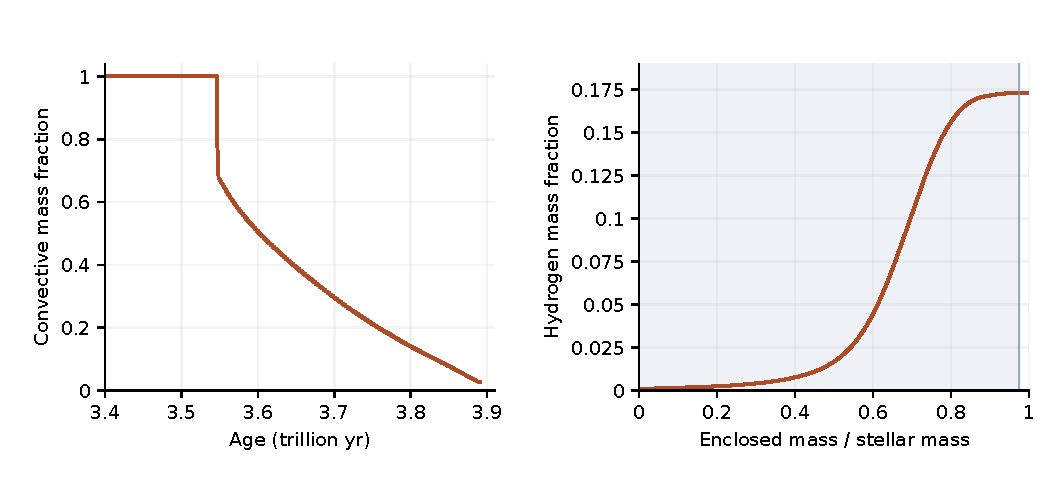
\includegraphics[width=0.7\textwidth]{convection_current.pdf}
\caption{Composition and convection histories. Upper: central (solid) and surface (dashed)
hydrogen for Track S (orange) and Track F (gray), with the LBA97 curve in
pale blue; the arrow follows increasing age along the Track S surface curve.
Lower: hydrogen and $^3$He in Track P (orange) against the LBA97 inset (pale
curves, read from the printed figure; diamonds mark LBA97's stated $^3$He
maximum and the hydrogen abundance at radiative-core formation). Crosses
show the reading precision of four image pixels, about $0.05\Tyr$ and 0.01
in mass fraction. Ages are shown as reported, without rescaling. Lower:
Track P's convective mass fraction, declining from unity near $3.546\Tyr$
to 0.02565 at $3.890\Tyr$, and its hydrogen profile at $3.890\Tyr$; the
shaded core carries heat by radiation and conduction.}
\label{fig:composition}
\end{figure}

\subsection{The end of full convection and the conductive core}
Track P first departs from full convection near $3.546\Tyr$ at central
$X=0.1751$: a radiative layer separates the convective centre from the
envelope. By $3.560\Tyr$ the convective mass fraction has fallen to 0.6277
and central hydrogen to 0.1518 while the surface remains at 0.1747, so the
star is no longer mixed as a whole. In Track F the same transition occurs
near $3.549\Tyr$ (3230 K, central $X=0.1744$) and the central convective
region disappears near $3.551\Tyr$. At that transition carbon-12 depletion
is 0.02652, with 0.02524 accumulated as carbon-13 and only 0.001275
converted to nitrogen: the two proton captures cannot be treated as an
instantaneous conversion of carbon to nitrogen during this phase.

At $3.890\Tyr$ Track P has a core containing 97.43\% of the mass that
carries heat by radiation and conduction beneath a convective envelope.
Central hydrogen is $8.157\times10^{-4}$ while the envelope remains near
0.1730. Conduction supplies 91.29\% of the central heat flux; in Track S at
$3.688\Tyr$ electron conduction supplies 99.79\%, with conductive and
radiative coefficients of $1.058\times10^{14}$ and $2.221\times10^{11}$
erg cm$^{-1}$ s$^{-1}$ K$^{-1}$ and a central degeneracy parameter of
15.39. The composition gradient also suppresses convection.
``Fully convective'' describes where convection occurs, not the fraction of
the luminosity it carries; radiation, conduction and convection share the
heat flow continuously, and the mixing-length treatment makes the convective
share go to zero at a stability boundary. Chemical mixing uses the stronger
approximation that each connected convective region becomes uniform quickly.

During the transition in Track F, a mainly radiative layer at enclosed mass
fractions 0.1770--0.2391 separates a convective core from the envelope.
Conduction supplies 4.4--4.8\% of its diffusive heat flow, yet removing
conductivity on that fixed structure would make the layer unstable under the
Ledoux criterion: conduction matters for the convection threshold even where
radiation carries most of the heat.

\subsection{What settling and diffusion change}
At their respective luminosity maxima, Track S is 26.13\% more luminous and
10.03\% smaller than Track F (Table~\ref{tab:lmax}), with nearly equal
central temperatures. Figure~\ref{fig:peak} compares the structures. Near
$3.673\Tyr$ the layer enclosing 80\% of the mass is hotter and denser with
settling, 8.260 rather than 7.402 MK and 489.6 rather than 245.0 g
cm$^{-3}$, and poorer in hydrogen, $X=0.1726$ rather than 0.2712; integrating
the reaction rates gives 27.25\% more nuclear power. Track S has consumed
0.4987\% more hydrogen than Track F at this point (80.83\% against 80.43\% of
the initial inventory). CN reactions contribute 1.286\% of its nuclear
power. The coupled tracks do not isolate the separate contributions of
atmospheric opacity, interior material properties and diffusion.

\begin{table}[H]\centering\small
\caption{Structure at the luminosity maximum.}\label{tab:lmax}
\begin{tabular}{@{}lrr@{}}\toprule
 & Track F & Track S \\\midrule
Age (Tyr) & 3.677 & 3.673 \\
Luminosity ($\Ls$) & 0.005163 & 0.006513 \\
Effective temperature (K) & 3695 & 4128 \\
Radius ($\Rs$) & 0.1753 & 0.1578 \\
Central temperature (MK) & 11.90 & 11.97 \\
Remaining hydrogen ($\Ms$) & $\simeq0.01370$ & 0.01342 \\
Convective mass fraction & 0.05536 & 0.03339 \\\bottomrule
\end{tabular}
\end{table}

\begin{figure}[H]\centering
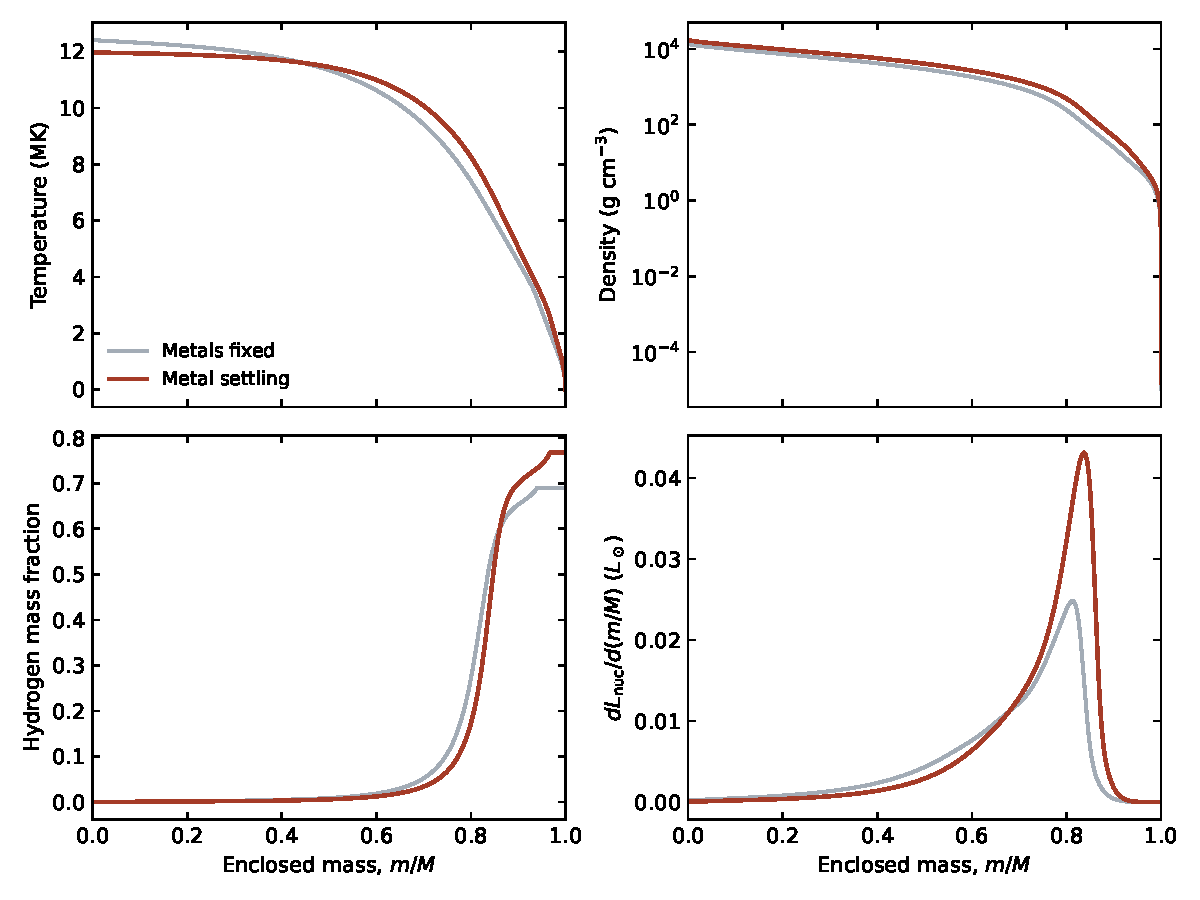
\includegraphics[width=0.93\textwidth]{metal_peak_structure.pdf}
\caption{Temperature, density, hydrogen abundance and nuclear power per unit
fractional mass at the Track S luminosity maximum, compared with a Track F
structure of nearly the same age (0.1837 Gyr later; not the Track F
maximum). The strongest burning occurs outside the depleted centre. The
curves compare actual structures; exchanging their profiles would not
produce equilibrium models.}
\label{fig:peak}
\end{figure}

\paragraph{Diffusion alone.}
A paired comparison from the same $3.560\Tyr$ Track F structure, evolved
50 Gyr with and without microscopic drift, gives central $X=0.02300$ with
drift and 0.06864 without, surface $X=0.2907$ and 0.1847, and effective
temperatures of 3404 and 3302 K. Total remaining hydrogen differs by only
0.2767\%, but the diffusive calculation burns 4.241\% more hydrogen during
the interval and ends 20.10\% more luminous. Over this interval diffusion
mainly redistributes fuel and changes the structure that burns it. Ember's
drift speeds at 14 weakly degenerate interfaces are 0.8163--0.9258 of the
classical Thoul--Bahcall--Loeb values \cite{thoul94}; the degenerate core
needs the actual gravity and electron thermodynamics \cite{paxton18}.

For a nearly homogeneous radiative centre, a drift speed of order
$Dm_pg/(kT)$ gives a separation time
\begin{equation}
 t_{\rm sep}\sim\frac{kT}{4\pi G\rho m_pD},
\end{equation}
of order 100 Gyr at $T\sim9$ MK, $\rho\sim300$ g cm$^{-3}$ and
$D\sim0.7$ cm$^2$ s$^{-1}$. Separation therefore competes with the final
core-burning phase while having little effect during the much longer fully
convective phase. The residual-fuel scale
\begin{equation}
 t_{\rm fuel}\sim10^{12}\,{\rm yr}\left(\frac{\Delta M_{\rm H}}{10^{-3}\Ms}\right)
 \left(\frac{L}{10^{-4}\Ls}\right)^{-1}
\end{equation}
shows why a central hydrogen threshold alone does not fix the duration of
shell burning: the energy is available only if hydrogen reaches layers hot
enough to burn, and diffusion controls that supply. LBA97 held the envelope
composition nearly fixed after the radiative core formed and included no
microscopic diffusion; its final whole-star hydrogen fraction is slightly
above 0.01 while its envelope retains $X=0.155$. The tracks here differ from
it in exactly the process that decides how much of that envelope hydrogen
ever burns.

\paragraph{Settling of metals.}
In Track S the surface-connected convective envelope shrinks from 4.716\%
of the mass at $3.664\Tyr$ to 2.013\% at $3.727\Tyr$ while its hydrogen
fraction rises from 0.6804 to 0.9945; helium and metals diffuse downward
through its base and the envelope ends nearly metal-free. A passive
calculation following C, N, O, Na, Mg, Si, Ca and Fe on the Track F
structures from 3.551 to $3.704\Tyr$, with the published collision
coefficients \cite{thoul94}, leaves surface abundances at 0.06213--0.08217
of their initial values with classical heat flow and 0.2491--0.3076 with heat
flow suppressed; the two treatments are alternative approximations, not an
uncertainty band. Halving the time interval changes the surface results by
at most 0.2078\%. Metals accumulate in the conductive core, reaching
$Z=0.1312$ at the Track S endpoint. Accretion could maintain surface metals
against settling \cite{bauer19}; the isolated model has none.

Removing metals from the atmosphere changes the boundary condition
appreciably. At $X=0.85$, 3800 K and $\log g=4.9$, reducing carbon and
nitrogen to 0.1531 and 0.1541 of their initial abundances (the Track F
surface values at $3.697\Tyr$) changes the joining temperature by $+3.314\%$
and the gas pressure by $-4.205\%$; halving all metals changes them by
$-8.606\%$ and $+53.69\%$. Applied as fixed boundary factors to the same
$3.694\Tyr$ structure for 100 Myr, the two changes give
$\Delta\Teff=-30.38$ K and $+142.9$ K, $\Delta L/L=-1.019\%$ and
$+5.041\%$, and $\Delta R/R=+1.142\%$ and $-4.983\%$. These establish an
appreciable surface-temperature response; the actual response in Track S
comes from the transported metal abundance and the metal-dependent
atmosphere families.

\subsection{Measured sensitivities}
Table~\ref{tab:sensitivity} collects the largest effect found for each
class of numerical or table approximation used along Track S. Each entry is
a paired comparison over the stated interval; none is a bound on the full
lifetime. The one entry that is not small is the absolute normalization of
the pure-hydrogen boundary, which is the subject of Section~\ref{sec:flash}.

\begin{table}[H]\centering\small
\caption{Largest measured sensitivities along Track S.}\label{tab:sensitivity}
\begin{tabular}{@{}p{0.36\textwidth}p{0.26\textwidth}p{0.32\textwidth}@{}}\toprule
Approximation tested & Largest table-level discrepancy & Largest stellar response (interval) \\\midrule
Atmosphere interpolation between solved columns (all families, Appendix Table~\ref{tab:atm}) & 2.031\% in $T$, 4.656\% in $P$ at the joining depth & 12.74 K, 0.3110\% in $L$ (30 Gyr) \\
Gravity continuation of the boundary, $\log g=5.95$--6.1 & 0.1878\% in $T$, 2.391\% in $P$ against nine solved atmospheres & 8.697 K, 0.5101\% in $L$ for $\pm0.5\%$/$\pm5\%$ offsets (50 Myr); 60.96 Gyr of track lies inside \\
Temperature continuation of the boundary to 4600 K & solved 4600 K atmosphere agrees within 0.05\% & 17.54 K, 1.026\% in $L$ for $\pm1\%$/$\pm10\%$ offsets (50 Myr) \\
Pure-hydrogen boundary: TLUSTY against the MESA table at 4600 K, $\log g=5.9$ & 2.594\% in $T$, 48.69\% in $P$ & about 241 K in 1 Myr (not converged; Section~\ref{sec:flash}) \\
Molecular opacity continuation below $Z=0.01$ & up to 9.237\% at $Z=0.003$ against withheld sources & 0.002433\% in $L$, 0.009728 K between linear and logarithmic forms (10 Gyr) \\
Radiative opacity $\pm10\%$ in the depleted envelope & --- & 0.6315\% in $L$, 3.216 K (1 Myr) \\
Warm interior opacity $\pm15\%$ (convective layers) & withheld-source differences up to 11.01\%; OPLIB 31.52--35.21\% & below $10^{-10}$ in $L$ and $R$ (1.25 Gyr) \\
Dense-core radiative opacity halved or doubled & --- & no significant change (25 Myr); conduction carries the heat \\
Variable-metal equation of state & 0.7642\% in $c_P$, 1.037\% in $\Gamma_1$ against FreeEOS & below 0.001 K (10 Myr) \\
Core equation of state to $Z=0.16$ & 0.07726\% in material state & 0.0004595 K, 0.0002080\% in $L$ (25 Myr) \\
Time-error tolerances threefold tighter & --- & 0.002872\% in $L$, 0.01705 K (5 Gyr) \\
Structure tolerance loosened to 0.001 & --- & 1.078\% in $L$, 3.114 K (2 Gyr); rejected \\\bottomrule
\end{tabular}
\end{table}
